\documentclass{article}
\usepackage[pdf]{graphviz}
\usepackage{graphviz}
\usepackage{amsmath}


\begin{document}

CS5200 Homework 2 Dynamic Programming\\
Adam McNeil\\
Question 1) \\
max heapify \\
\indent Call max heapify on all the internal nodes starting at the bottom \\
\indent maxHeapify(25) \\

\digraph[scale=0.5]{stepone}{
   node [shape=circle]
   edge [arrowhead=none]
   subgraph clusterGraph {
       label="maxHeapify(25)"
       array [shape=record label="10|20|60|30|70|29|25"]
       10 -> 20 
       10 -> 60
       20 -> 30
       20 -> 70
       60 -> 29
       60 -> 25 [dir="both" arrowhead=normal]
   }
   60 [color=red]
   25 [color=red]
}

\digraph[scale=0.5]{steptwo}{
   node [shape=circle]
   edge [arrowhead=none]
   subgraph clusterGraph {
       label="maxHeapify(20)"
       array [shape=record label="10|70|60|30|20|29|25"]
       10 -> 70 
       10 -> 60
       70 -> 30
       70 -> 20 [dir="both" arrowhead=normal]
       60 -> 29
       60 -> 25
   }
   70 [color=red]
   20 [color=red]
}

\digraph[scale=0.5]{stepthree}{
   node [shape=circle]
   edge [arrowhead=none]
   subgraph clusterGraph {
       label="maxHeapify(10)"
       array [shape=record label="70|30|60|10|20|29|25"]
       70 -> 30 [dir="both" arrowhead=normal]
       70 -> 60
       30 -> 10 [dir="both" arrowhead=normal]
       30 -> 20 
       60 -> 29
       60 -> 25
       
   }
   70 [color=red]
   30 [color=red]
   10 [color=red]
}

\digraph[scale=0.5]{delete}{
   node [shape=circle]
   edge [arrowhead=none]
   subgraph clusterGraph {
       label="delete(70)"
       array [shape=record label="25|30|60|10|20|29|70"]
       25 -> 30 
       25 -> 60
       30 -> 10 
       30 -> 20 
       60 -> 29
       
   }
   60 [color=red]
   29 [color=red]
   25 [color=red]
}

\digraph[scale=0.5]{stepfour}{
   node [shape=circle]
   edge [arrowhead=none]
   subgraph clusterGraph {
       label="maxHeapify(25)"
       array [shape=record label="60|30|29|10|20|25|   "]
       60 -> 30 
       60 -> 29
       30 -> 10 
       30 -> 20 
       29 -> 25
       
   }
   25 [color=red]
   60 [color=red]
   29 [color=red]
}

\digraph[scale=0.5]{insert}{
   node [shape=circle]
   edge [arrowhead=none]
   subgraph clusterGraph {
       label="insert(80)"
       array [shape=record label="60|30|29|10|20|25|80"]
       60 -> 30 
       60 -> 29
       30 -> 10 
       30 -> 20 
       29 -> 25
       29 -> 80
       
   }
   80 [color=red]
}

\digraph[scale=0.5]{insertHeapify}{
   node [shape=circle]
   edge [arrowhead=none]
   subgraph clusterGraph {
       label="maxHeapify(60)"
       array [shape=record label="80|30|60|10|20|25|29"]
       80 -> 30 
       80 -> 60 [dir="both" arrowhead=normal]
       30 -> 10 
       30 -> 20 
       60 -> 25
       60 -> 29 [dir="both" arrowhead=normal]
       
   }
   60 [color=red]
   29 [color=red]
   80 [color=red]
} \\

\digraph[scale=0.5]{heapSort}{
   node [shape=circle]
   edge [arrowhead=none]
   subgraph clusterGraph {
       label="heapSort()"
       array [shape=record label="29|25|20|10|30|60|80"]
       29 -> 25 
       29 -> 20 
       25 -> 10
       
   }

} \\


Question 2) 
\digraph[scale=0.5]{questiontwo}{
    node [shape=circle]
    edge [arrowhead=none]
    72 -> {35, 91}
    35 -> {18, 37}
    91 -> {83, 92}
    18 -> {1, 19} 
    37 -> {2, 62}
    
    1 [shape=point]
    2 [shape=point]
}\\
% Pre-order = root left right
% In-order = left root right
% Post-order = left right root
\indent Pre-order: 72 35 18 19 37 62 91 83 92 \\
\indent In-order: 18 19 35 37 62 72 83 91 92 \\
\indent Post-order: 19 18 62 37 35 83 92 91 72 \\

\digraph[scale=0.5]{btinsertone}{
    label="insert(13)"
    node [shape=circle]
    edge [arrowhead=none]
    72 -> {35, 91}
    35 -> {18, 37}
    91 -> {83, 92}
    18 -> {13, 19} 
    37 -> {2, 62}
    
    2 [shape=point]
}

\digraph[scale=0.5]{btinsertwo}{
    label="insert(40)"
    node [shape=circle]
    edge [arrowhead=none]
    72 -> {35, 91}
    35 -> {18, 37}
    91 -> {83, 92}
    18 -> {13, 19} 
    37 -> {2, 62}
    62 -> {40, 1}
    
    1 [shape=point]
    2 [shape=point]
}

\digraph[scale=0.5]{btdelete}{
    label="delete(35)"
    node [shape=circle]
    edge [arrowhead=none]
    72 -> {37, 91}
    91 -> {83, 92}
    18 -> {13, 19} 
    37 -> {18, 62}
    62 -> {40, 1}
    
    1 [shape=point]
}\\
Question 3) \\
$ p_{0} = 4 \,\  p_{1} = 10 \,\  p_{2} = 3 \,\  p_{3} = 12 \,\  p_{4} = 7 $\\

\begin{tabular}{ c | c | c | c | c }
            
    & 1 & 2 & 3 & 4 \\ 
  4 & 0 & 0 & 252 & 0 \\  
  3 & 0 & 360 & 0 \\
  2 & 120 & 0 \\
  1 & 0     
\end{tabular}
\begin{tabular}{ c | c | c | c | c }
            
    & 1 & 2 & 3 & 4 \\ 
  4 &   &   & 3 & 0 \\  
  3 &   & 2 & 0 \\
  2 & 1 & 0 \\
  1 & 0     
\end{tabular}\\

    \textbf{m(1, 3) i=1 j=3} \\
    k=1 \\
    m(1, 1) + m(2, 3) + $ p_{0}\ p_{1}\  p_{3}$\\
    0 + 360 + 4*10*12 = 840 \\\\

    k=2 \\
    m(1, 2) + m(3, 3) + $ p_{0}\ p_{2}\  p_{3}$\\
    120 + 0 + 4*3*12 = 264\\\\

    \textbf{m(2, 4) i=2 j=4} \\
    k=2 \\
    m(2, 2) + m(3, 4) + $ p_{1}\ p_{2}\  p_{4}$\\
    0 + 252 + 10*3*7 = 462 \\\\

    k=3 \\
    m(2, 3) + m(4, 4) + $ p_{1}\ p_{3}\  p_{4}$\\
    120 + 0 + 10*12*7 = 462\\\\

    \begin{tabular}{ c | c | c | c | c }
            
        & 1 & 2 & 3 & 4 \\ 
    4 & 0 & 462 & 252 & 0 \\  
    3 & 264 & 360 & 0 \\
    2 & 120 & 0 \\
    1 & 0     
    \end{tabular}
    \begin{tabular}{ c | c | c | c | c }
            
        & 1 & 2 & 3 & 4 \\ 
      4 &   & 2 & 3 & 0 \\  
      3 & 2 & 2 & 0 \\
      2 & 1 & 0 \\
      1 & 0     
    \end{tabular}\\

    \textbf{m(1, 4) i=1 j=4} \\
    k=1 \\
    m(1, 1) + m(2, 4) + $ p_{0}\ p_{1}\  p_{4}$\\
    0 + 462 + 4*10*7 = 742 \\\\

    k=2 \\
    m(1, 2) + m(3, 4) + $ p_{0}\ p_{2}\  p_{4}$\\
    120 + 252 + 4*3*7 = 456\\\\

    k=3 \\
    m(1, 3) + m(4, 4) + $ p_{1}\ p_{3}\  p_{4}$\\
    264 + 0 + 4*12*7 = 600\\\\

    \begin{tabular}{ c | c | c | c | c }
            
        & 1 & 2 & 3 & 4 \\ 
    4 & 456 & 462 & 252 & 0 \\  
    3 & 264 & 360 & 0 \\
    2 & 120 & 0 \\
    1 & 0     
    \end{tabular}
    \begin{tabular}{ c | c | c | c | c }
            
        & 1 & 2 & 3 & 4 \\ 
      4 & 2 & 2 & 3 & 0 \\  
      3 & 2 & 2 & 0 \\
      2 & 1 & 0 \\
      1 & 0     
    \end{tabular}\\
 $ (A_{1} \  A_{2}) \  (A_{3} \ A_{4}) $\\
 Question 4)   \\
    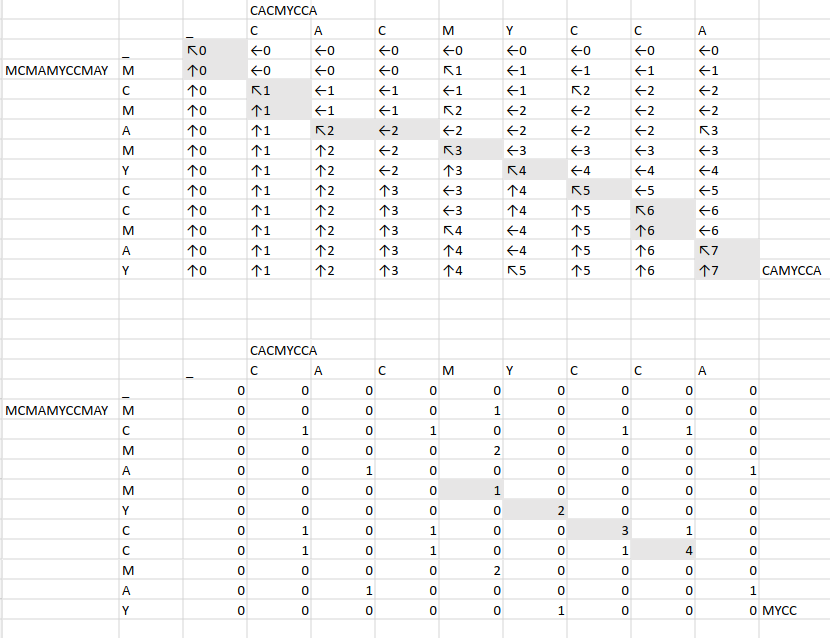
\includegraphics[scale=0.5]{subsequence.png}
Question 5)\\
\begin{tabular}{ c | c | c | c | c | c}         
          i & 0 & 1 & 2 & 3 & 4 \\ 
\hline    $p_{i}$ & 0 & 0.05 & 0.12 & 0.3 & 0.2 \\  
\hline    $q_{i}$ & 0.07 & 0.07 & 0.07 & 0.06 & 0.06 \\
\end{tabular}
\\\\

w[i, j] = w[i, j-1] + $p_{j}$ + $q_{j}$\\
\\
w[1, 1] = w[1, 0] + $p_{1}$ + $q_{1}$ = 0.07 + 0.05 + 0.07 = 0.19 \\
w[3, 2] = w[3, 1] + $p_{2}$ + $q_{2}$ = 0.26 + 0.30 + 0.06 = 0.62 \\
w[4, 4] = w[4, 3] + $p_{4}$ + $q_{4}$ = 0.06 + 0.20 + 0.06 = 0.32 \\

\begin{tabular}{ c | c | c | c | c | c}         
w & 1 & 2 & 3 & 4 & 5 \\ 
\hline 4 & 1.00 & 0.88 & 0.69 & 0.32 & 0.06 \\  
\hline 3 & 0.74 & 0.62 & 0.43 & 0.06 \\
\hline 2 & 0.52 & 0.26 & 0.07 \\
\hline 1 & 0.19 & 0.07 \\   
\hline 0 & 0.07        
\end{tabular}

r is from i to j \\
save the lowest r to root table and record the lowest value in the c table\\
c[i, j] = c[i, r-1] + c[r+1, j] + w[i, j]\\
\\
\textbf{r = 1} \\
c[1, 1] = c[1, 0] + c[2, 1] + w[1, 1] = 0.07 + 0.07 + 0.19 = 0.33\\
\\
\textbf{r = 1} \\
c[1, 2] = c[1, 0] + c[2, 2] + w[1, 2] = 0.07 + 0.40 + 0.52 = 0.99\\
\textbf{r = 2} \\
c[1, 2] = c[1, 1] + c[3, 2] + w[1, 2] = 0.33 + 0.07 + 0.52 = 0.92\\

\begin{tabular}{ c | c | c | c | c | c}         
c & 1 & 2 & 3 & 4 & 5 \\ 
\hline 4 & 2.36 & 1.76 & 1.20 & 0.44 & 0.06 \\  
\hline 3 & 1.63 & 1.08 & 0.56 & 0.06 \\
\hline 2 & 0.92 & 0.40 & 0.07 \\
\hline 1 & 0.33 & 0.07 \\   
\hline 0 & 0.07     
\end{tabular}
\\ \\
\begin{tabular}{ c | c | c | c | c | c}         
root & 1 & 2 & 3 & 4  \\ 
\hline 4    & 3 & 3 & 3 & 4 \\  
\hline 3    & 2 & 3 & 3 \\
\hline 2    & 2 & 2 \\
\hline 1    & 1 \\   
\end{tabular}
\\
Bonus:\\
optimal substructure the solution either contains the number or does not contain the number\\
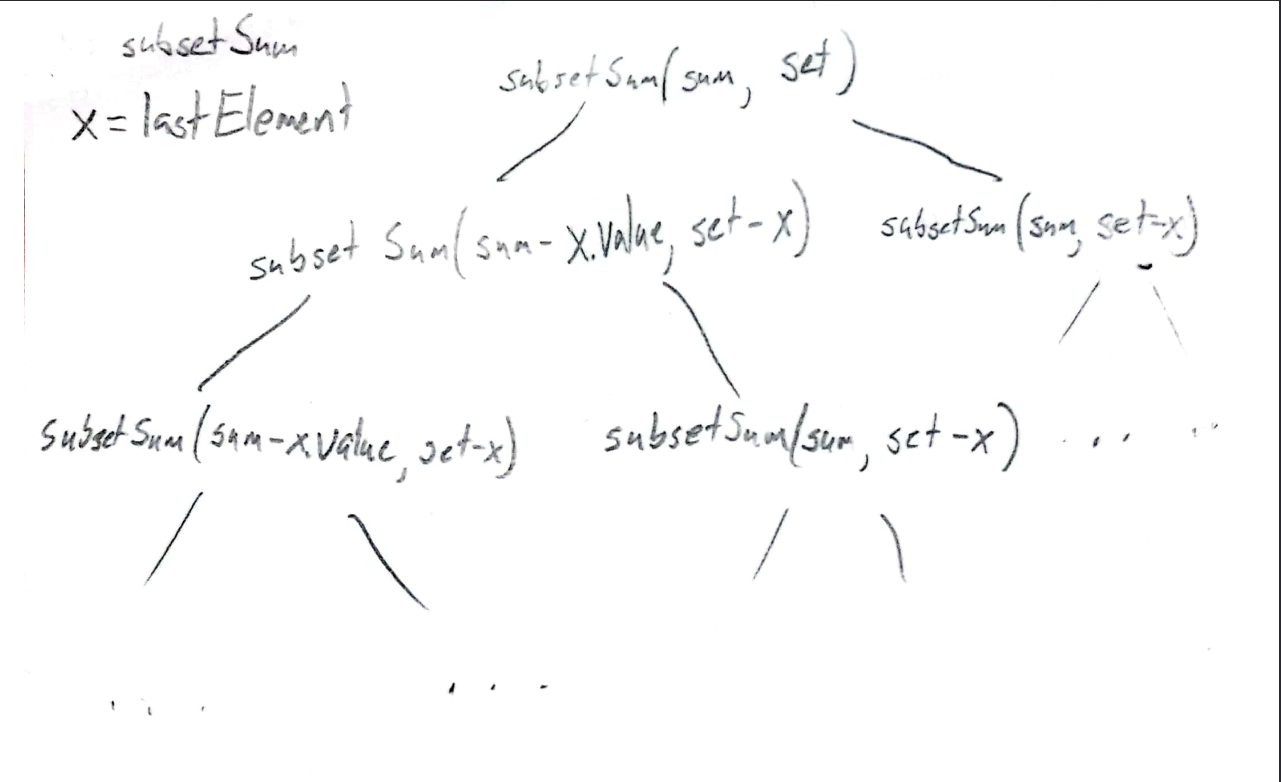
\includegraphics[scale=0.25]{graph.png}

Pseudo code: \\ 
sumOfSubset(set, n) {\\
\indent listOfSums = [0]\\
\indent for i in set:\\
\indent \indent for j in listOfSums:\\
\indent \indent \indent if i + j is not in listOfSums:\\
\indent\indent\indent\indent listOfSums.addFront(i+j)\\
\indent return is n in listOfSums\\
}
\end{document}